\subsection{Tempo di esecuzione}

Nel calcolare il tempo di esecuzione di un algoritmo parallelo, la grandezza nota come complessità di tempo (utile nell'analisi del tempo di esecuzione di un algoritmo sequenziale) risulta poco indicativa.\\
Infatti, in un algoritmo parallelo il numero delle operazioni non coincide più con il numero dei passi temporali. Di conseguenza si introducono nuove grandezze al fine di realizzare un'analisi degli algoritmi paralleli.

In un ambiente di calcolo parallelo con P che indica il numero di processori, un problema che si risolve in un tempo T verrà risolto da P processori (idealmente) in $\frac{T}{P}$.


\subsection{Speed-up, Overhead ed Efficienza}

Lo \textbf{speed-up} misura la riduzione del tempo di esecuzione rispetto all'algoritmo sequenziale ed è definito dal rapporto:
$$ S(P) = \frac{T(1)}{T(P)} $$ 


La quantità che misura quanto il nostro speed up differisce da quello ideale è l'overhead. Si può quantificare con la seguente formula: $O_h(p) = pT(p) - T(1)$ .\\
Riscrivendo lo speed up in funzione dell'overhead ci accogiamo infatti che lo speed up è ideale se e solo se l'overhead è nullo.\\

Per poter misurare se e quanto è stato "sfruttato" il nostro ambiente di calcolo parallelo, si introduce l' \underline{efficienza} del nostro algoritmo.
Si definisce \textbf{efficienza} il rapporto: $$ E(p) = \frac{S(p)}{p} $$

\subsection{Dati empirici}
L'algoritmo è stato testato in più condizioni e secondo i parametri precedentemente descritti.

Avendo fissato ad un milione la dimensione del problema ed avendo fatto variare il numero di processori da 2 a 8 (per il caso di singolo processore, si è deciso di eseguire l'algoritmo sequenziale per la somma), tenendo conto esclusivamente delle potenze di 2, sono stati ottenuti i seguenti risultati:

É stato fissata una dimensione di 1000x1000 per la matrice in input e di 1000 per il vettore.
Il numero di thread é variato da 1 a 8, tenendo conto delle sole potenze di 2.

\begin{table}[htp]
\centering
%\caption{}
\begin{tblr}{
  hlines,
  vlines,
}
Threads & Tempo ($\cdot 10^{-3} s$) & Speed Up & Efficienza & Overhead ($\cdot 10^{-3} s$) \\
1          & x   & x    & x       & x                     \\
2          & x   & x    & x       & x                     \\
4          & x   & x    & x       & x                     \\
8          & x   & x    & x       & x                     
\end{tblr}
\end{table}


\clearpage

Il grafico dei tempi:
\begin{figure}[h!tbp]
    \centering
    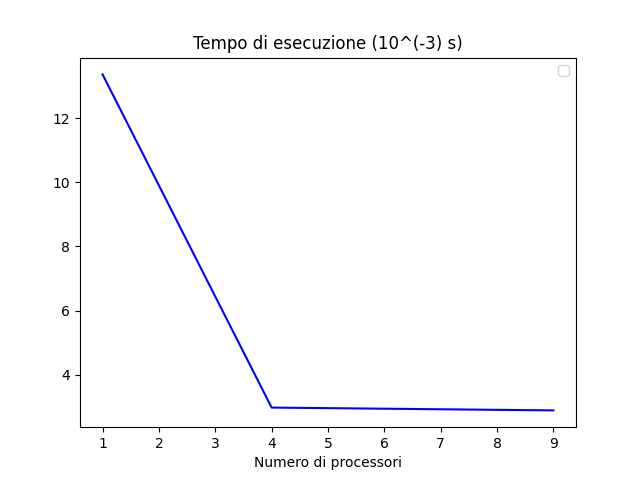
\includegraphics[width=1\linewidth]{Tempi.png}
    \caption{Andamento dei tempi}
    \label{fig:enter-label}
\end{figure}

\newpage
Visualizziamo la curva, confrontandola all'andamento dello speed-up ideale:
\begin{figure}[h!tbp]
    \centering
    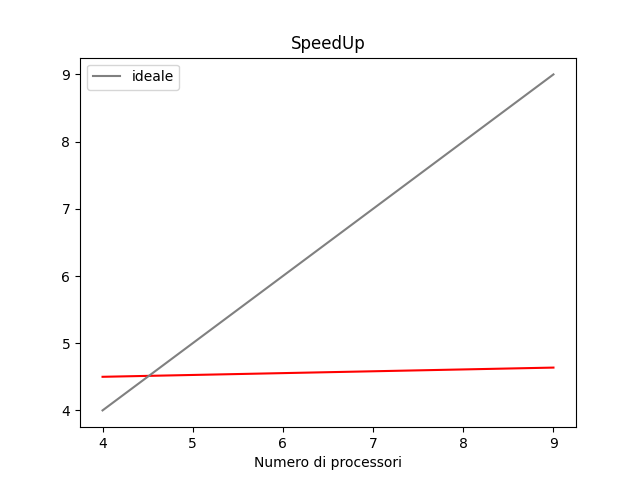
\includegraphics[width=1\linewidth]{SpeedUp.png}
    \caption{Andamento dello Speed Up}
    \label{fig:enter-label}
\end{figure}
\clearpage
Visualizziamo su un grafico anche i valori dell'Overhead:

\begin{figure}[h!tbp]
    \centering
    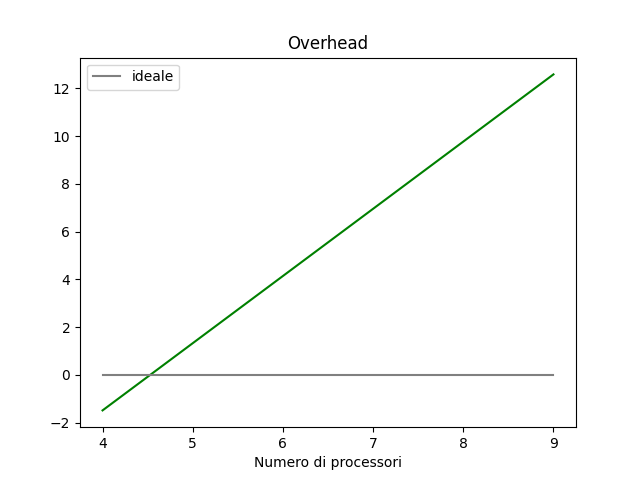
\includegraphics[width=1\linewidth]{Overhead.png}
    \caption{Andamento dell'Overhead}
    \label{fig:enter-label}
\end{figure}

\clearpage

Infine osserviamo come varia la nostra efficienza:
\begin{figure}[h!tbp]
    \centering
    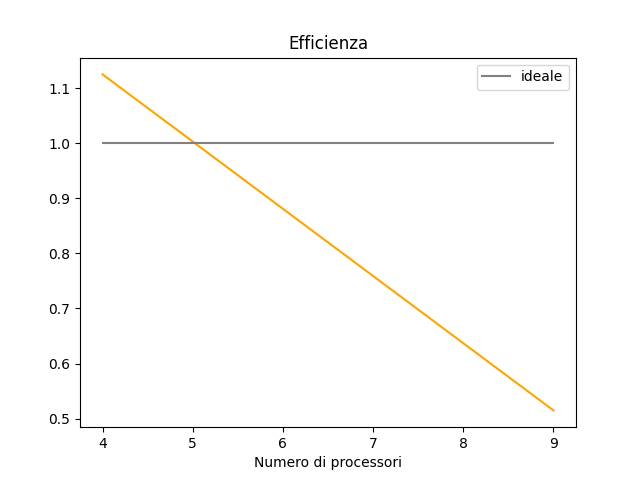
\includegraphics[width=1\linewidth]{Efficienza.png}
    \caption{Andamento dell'efficienza}
    \label{fig:enter-label}
\end{figure}